\chapter{Mobility Support}
\label{mobility support}

\section{Motivation for Mobility Support}

TCP/IP has 3 loosely-connected protocol layers running on top of physical
networking technologies.

\begin{figure}[H]
  \centering
  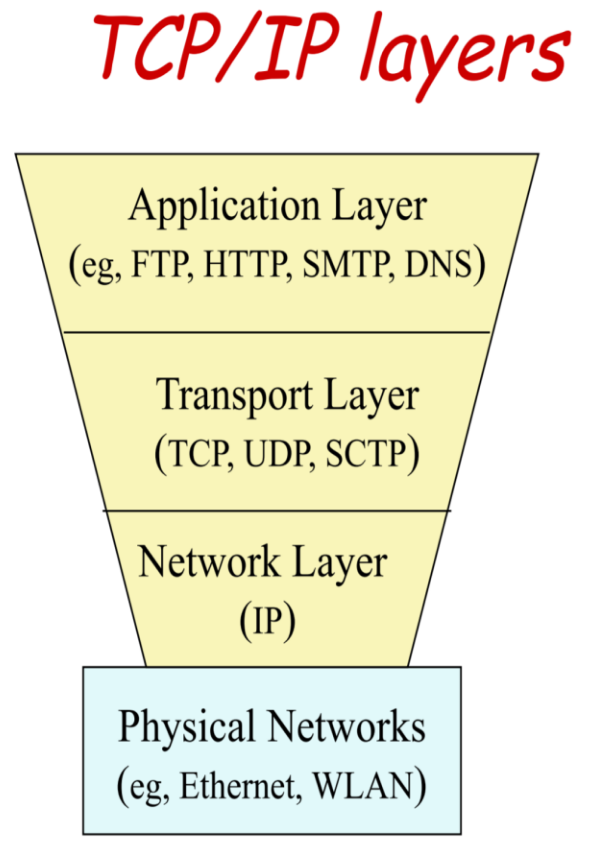
\includegraphics[scale=0.2]{tcp_ip_layers.png}
  \caption{TCP/IP layers}
  \label{fig:tcpiplayers}
\end{figure}

\textbf{Routing in the Internet}

\begin{itemize}
\item prefix-based routing: IP destination address and network prefix (e.g.
129.13.42) determines physical subnet
\item change of physical subnet implies change of IP address in order to have a
topological correct address
\item IP address is bound to a location (\textbf{point of attachment})
\end{itemize}

\textbf{Key Requirements of IP Mobility}

\begin{itemize}
\item \textbf{Reachability} - A mobile user must remain reachable at all times
via some permanent identifier regardless of its current location (\textbf{subnet
of attachment)}
\item \textbf{Continuity} - An ongoing communication should not break when the
mobile user moves (across subnet boundaries)
\end{itemize}

\textbf{Desirables requirements}

\begin{itemize}
\item \textbf{Compatibility} - No changes to current endsystems and routers
required
\item \textbf{Transparency} - Continuation of communication after interruption
of link possible
\item \textbf{Efficiency and scalability} - Little or no overhead (typical
connection via low bandwidth radio link)
\item \textbf{Security} - Authentication of all registration messages
\end{itemize}

\subsection{Problem and possible solution}

None of the layers was designed for mobility.
Mobile devices change IP address while crossing subnets and doesn't remain
reachable anymore.

IP address change breaks transport layer connections, so continuity is
weakened.\\

\textbf{Taxonomy}

\begin{itemize}
\item Scale: macro, micro
\item Entities involved in mobility management: mobile-assisted, network-only
\item Node or group mobility
\end{itemize}

How to handle mobility?\\

\textbf{Change the IP layer} so that the higher layers can still operate without
knowing you have moved (network layer solutions to mobility - e.g.,
MobileIP (v4, v6), GTP) or...

\textbf{Change TCP} so that it can cope with changing end-point identifiers
(transport layer solutions to mobility - e.g., Mobile TCP, SCTP).

\textbf{Root of the problem and an idea}: the IP address serves as both your
address that is used to locate you, and as your identity that is used to
identify you in TCP connections.

\subsection{Mobile IP}

\begin{figure}[H]
  \centering
  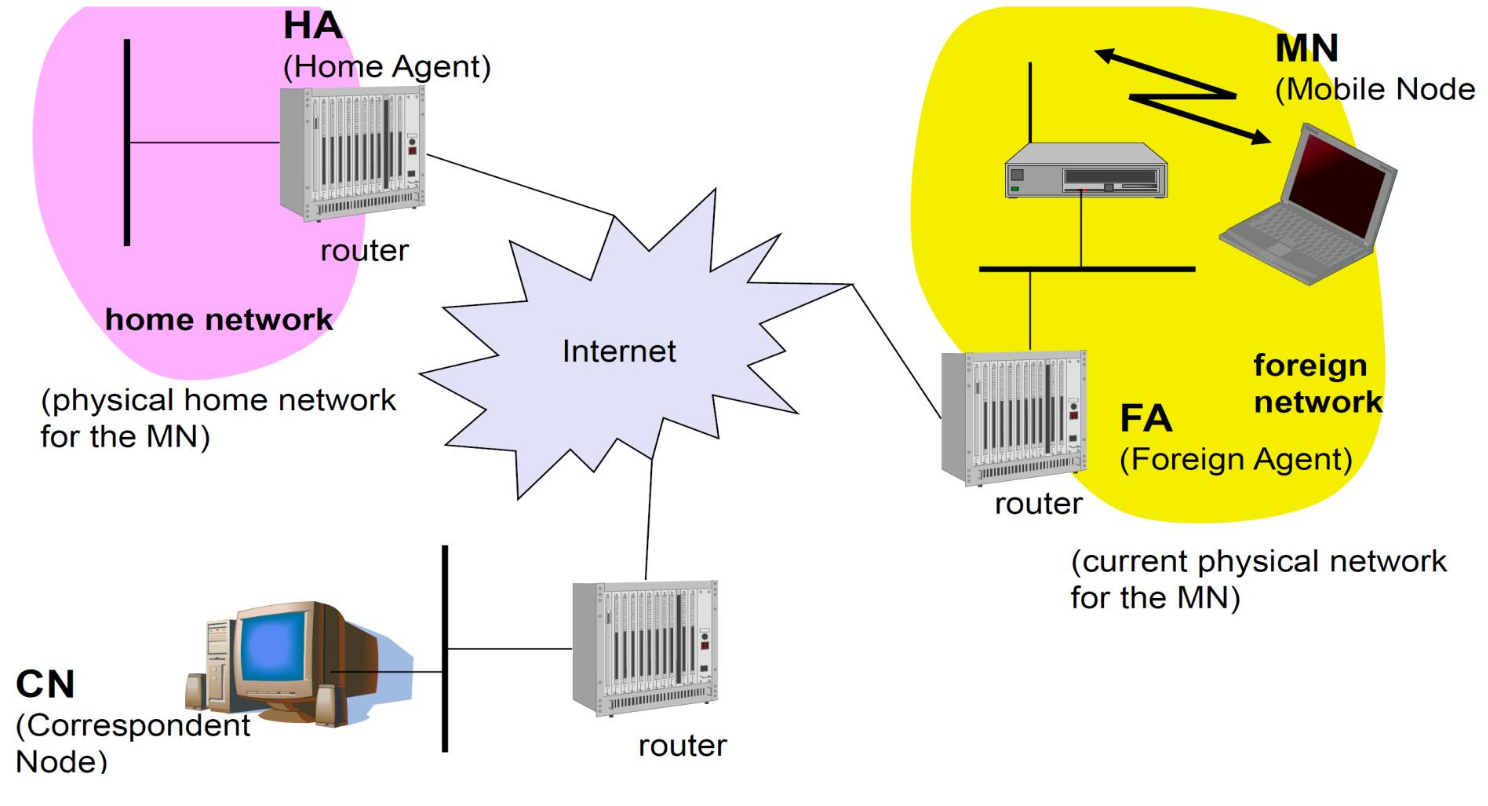
\includegraphics[scale=0.2]{mobileip1.png}
  \caption{Mobile IP example, entities involved}
  \label{fig:mobileip1}
\end{figure}

MN (Mobile Node) moves and senses a network change by listening to periodic
beacons transmitted by the FA (Foreign Agent).

The HA (Home Agent) maintains the binding (home address, care of address,
duration of validity).

Care of address: temporary IP for a mobile device.

\begin{figure}[H]
  \centering
  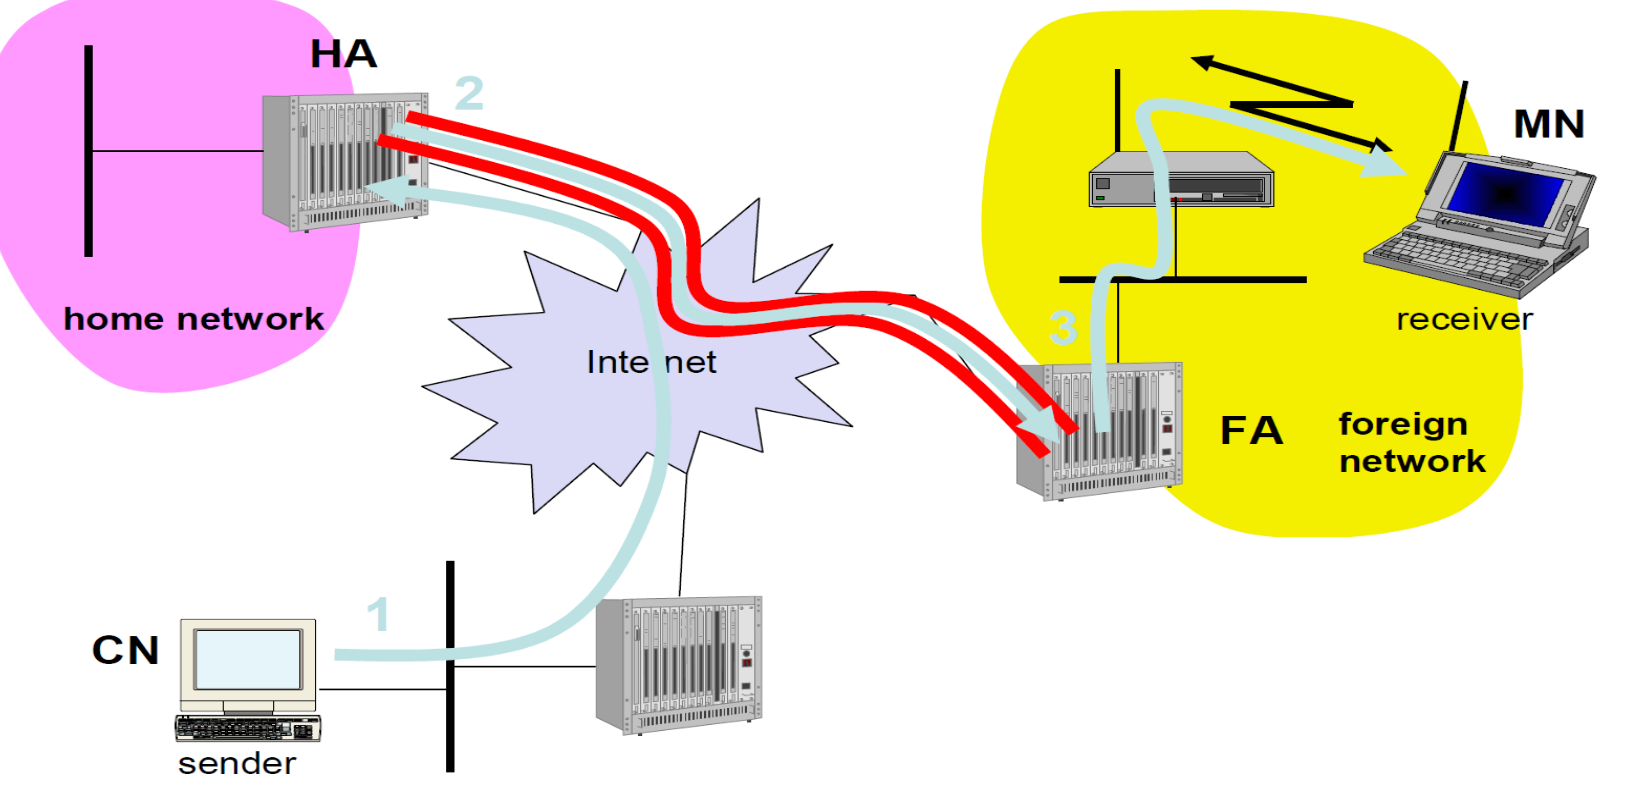
\includegraphics[scale=0.2]{mobileip2.png}
  \caption{Mobile IP example, CN -> MN}
  \label{fig:mobileip2}
\end{figure}

When any packets arrive at the home address, the Home Agent tunnels those
packets to the foreign agent / mobile node at its new address.

IP-in-IP tunneling means that the original IP packet is encapsulated in another
IP packet with the new destination address being the care of address.

\begin{figure}[H]
  \centering
  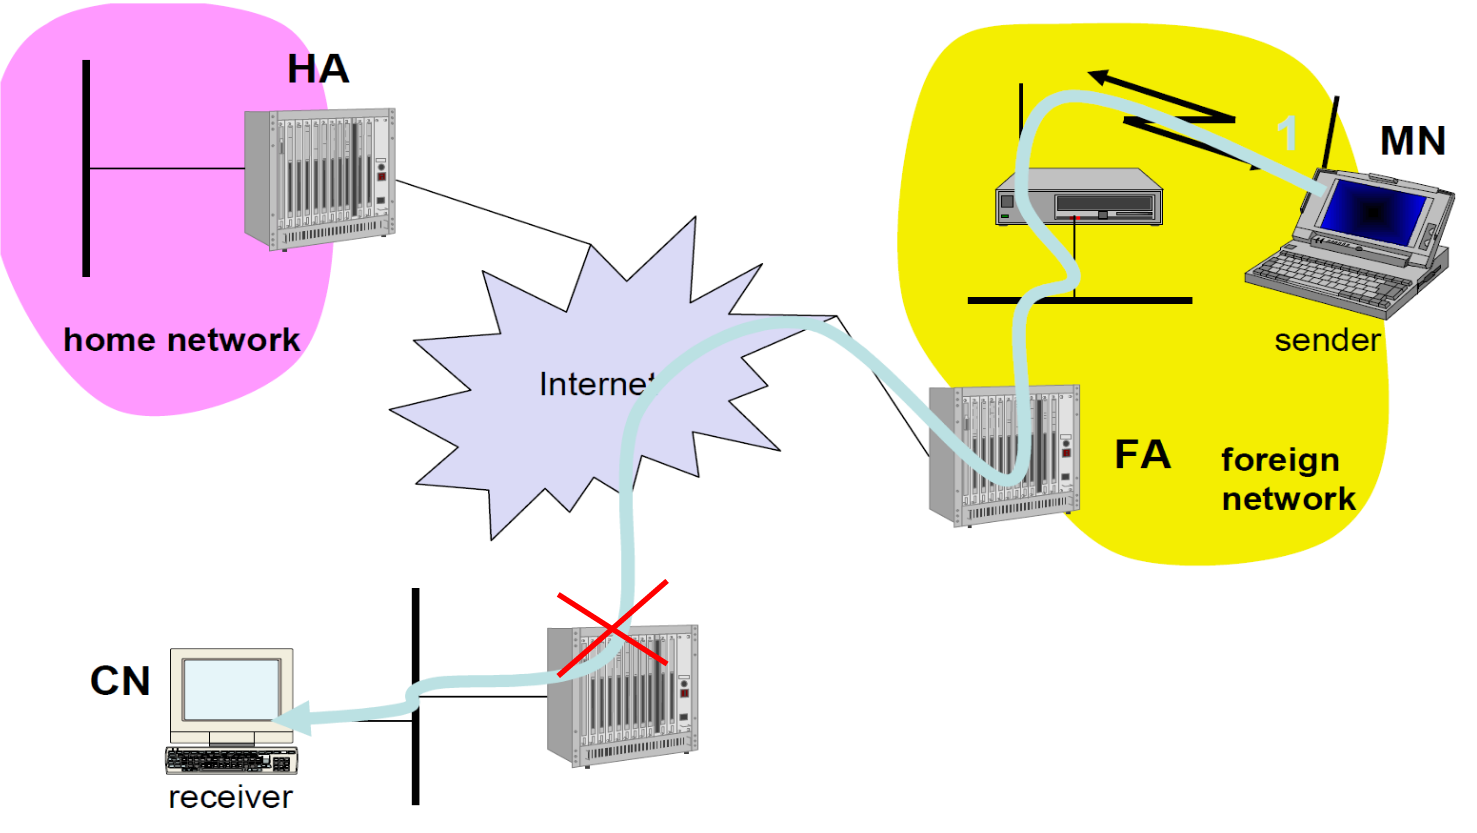
\includegraphics[scale=0.2]{mobileip3.png}
  \caption{Mobile IP example, MN -> CN}
  \label{fig:mobileip3}
\end{figure}

The mobile node can send replies directly, or reverse tunnel (i.e. firewall
scenario) them via home agent.\\

\textbf{Mobile IP - Cons}

\begin{itemize}
\item \textbf{Security} - Any malicious node can announce a new care of address
and steal packets. To prevent this, home agent and mobile node must share a
secret key and authenticate their communications
\item \textbf{Longer routes} - Packets have to travel extra distance
to the home agent and back (triangle routing).
MN could send the care of address (binding) to the CN (Correspondent Node)
which uses it subsequently -> security/privacy issues!
There is also a higher burden on the CN side
\item \textbf{Ingress filtering at routers}
ISPs can block packets coming from mobile nodes if the source address is their
old home address and does not belong to the IP block of its current network
\end{itemize}

\textbf{Mobile IP - Pros}

\begin{itemize}
\item Solves mobility at the root (IP is the lowest layer in TCP/IP)
\item In-built (integrato) tracking support (via permanent IP address and HA)
\item No change to network core (only edge routers - e.g., HA are affected)
\item Location privacy (no route optimization)
\end{itemize}

\textbf{Mobile IPv6}

\begin{itemize}
\item In IPv6, the foreign agent functionality is integrated into the IP stack
of the mobile node itself
\item Route Optimization is an integral part of the protocol
\item Built-in security
\end{itemize}

\section{Mobile Cellular Systems}

\subsection{Disambiguation}

\begin{enumerate}
\item E-UTRA(N) - Evolved UMTS Terrestrial Radio Access (Network)
\item Super 3G - Is referring to LTE, like WCDMA is referring to UTRA FDD and
TDD
\item 3.9G - Used to indicate that LTE is not 4G
\end{enumerate}

\textbf{Set of requirements issued by the ITU-R of the ITU in 2008 for what is
marketed as 4G}

\begin{itemize}
\item Based on an all-Internet Protocol (IP) packet switched network
\item Interoperability with existing wireless standards
\item A nominal data rate of 100 Mbit/s (while mobile) and 1 Gbit/s (while
client and station are in relatively fixed positions)
\item Dynamically share and use the network resources to support more
simultaneous users per cell
\item Scalable channel bandwidth 5–20 MHz, optionally up to 40 MHz
\item Peak link spectral efficiency of 15 bit/s/Hz in the downlink, and 6.75
bit/s/Hz in the uplink
\item Seamless (senza interruzioni) connectivity and global roaming across
multiple networks with smooth handovers (handoff)
\item System spectral efficiency of up to 3 bit/s/Hz/cell in the downlink and
2.25 bit/s/Hz/cell for indoor usage
\item Ability to offer high quality of service for multimedia support
\end{itemize}

\begin{figure}[H]
  \centering
  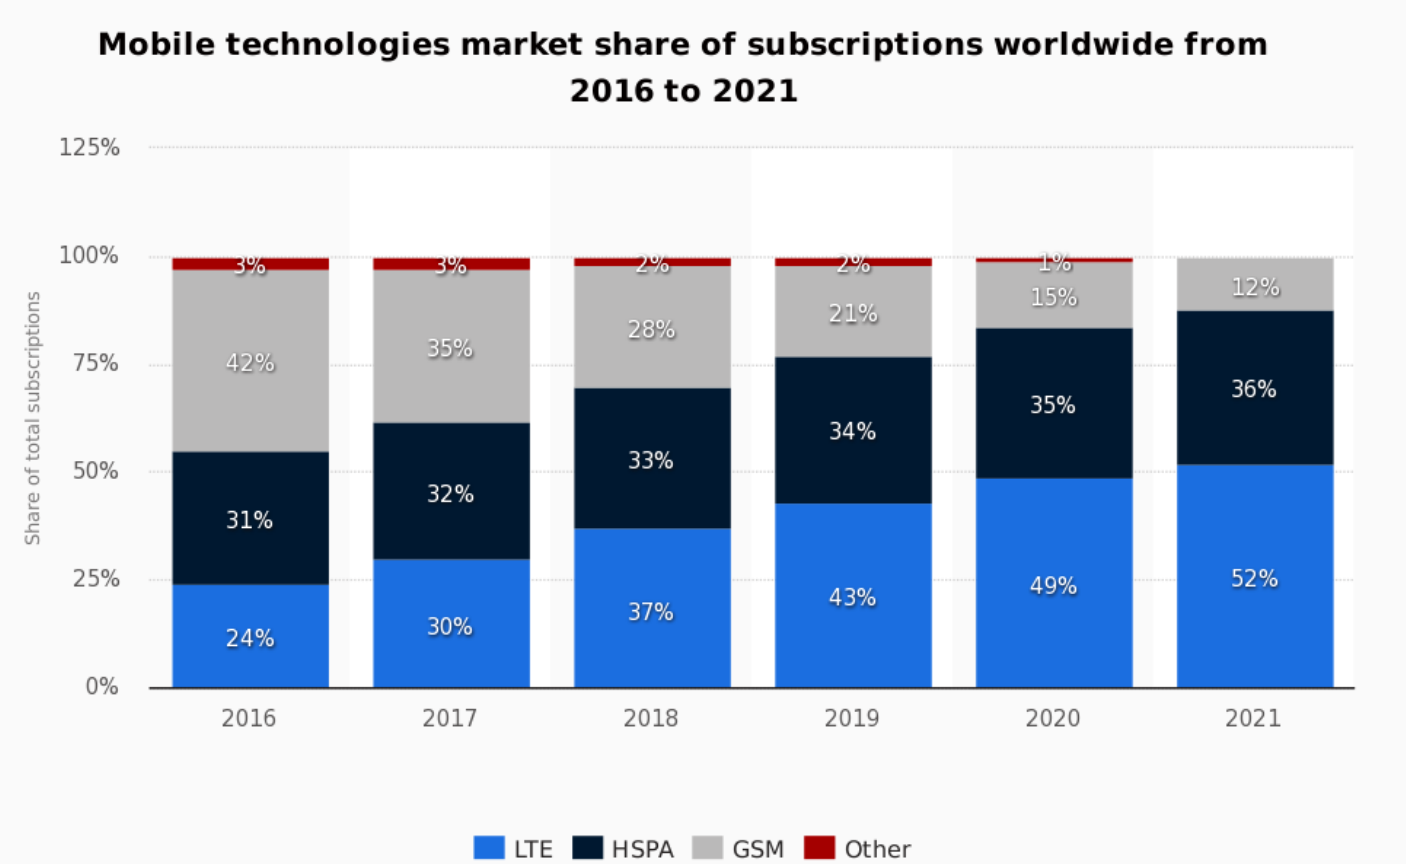
\includegraphics[scale=0.3]{mobtech.png}
  \caption{Mobile technologies market share of subscriptions worldwide from
  2016 to 2011}
  \label{fig:mobtech}
\end{figure}

\subsection{GSM}

\textbf{GSM (Global System for Mobile Communications)} is a standard
developed by the European Telecommunications Standards Institute (ETSI) to
describe the protocols for second-generation (2G) digital cellular networks
used by mobile phones.

As of 2014, it has become the de-facto global standard for mobile communications
with over 90\% market share, operating in over 219 countries and territories.

2G networks developed as a replacement for first generation (1G) analog cellular
networks, and the GSM standard originally described as a digital,
circuit-switched network optimized for full duplex voice telephony.

This expanded over time to include data communications, first by
circuit-switched transport, then by packet data transport via GPRS
(General Packet Radio Services) and EDGE (Enhanced Data rates for GSM Evolution,
or EGPRS).

Subsequently, the 3GPP developed third-generation (3G) UMTS standards, followed
by fourth-generation (4G) LTE Advanced standards, which do not form part of the
ETSI GSM standard.

\subsubsection{History...}

\textbf{1982 - Groupe Speciale Mobile is established}

\textbf{1989} - European Telecommunications Standardization Institute
(ETSI) takes over standardization and changes name: Global System for Mobile
(GSM) communication

\textbf{1990} - First Official Commercial launch in Europe

\textbf{1995} - GSM Specifications ported to 1900 MHz band \\

GSM is the most popular 2G technology. The following are its main
characteristics:

\begin{itemize}
\item FDD/FDMA/TDMA channel
\item TDMA: 200 KHz channel with 8 voice channels;
\item TDMA: channel rate of 270.833 kbps (~33 kbps per user);
\item TDMA: divided into two logical control and data channel (22.8kbps)
\item Higher Quality than prior analog systems
\item Digital Voice 13.3Kbps
\item 9.6 kbps for data traffic
\item Low power handsets – support sleep mode
\item Security through encryption
\item Wide roaming capability
\item Subscriber Identity Modules (SIM cards)
\item Digital data service
\item fax, circuit switched data
\item SMS short messaging service
\item Additional features such as call waiting, voice mail, group calling,
caller id etc.
\end{itemize}

\subsubsection{GSM – Functional Architecture}

\begin{figure}[H]
  \centering
  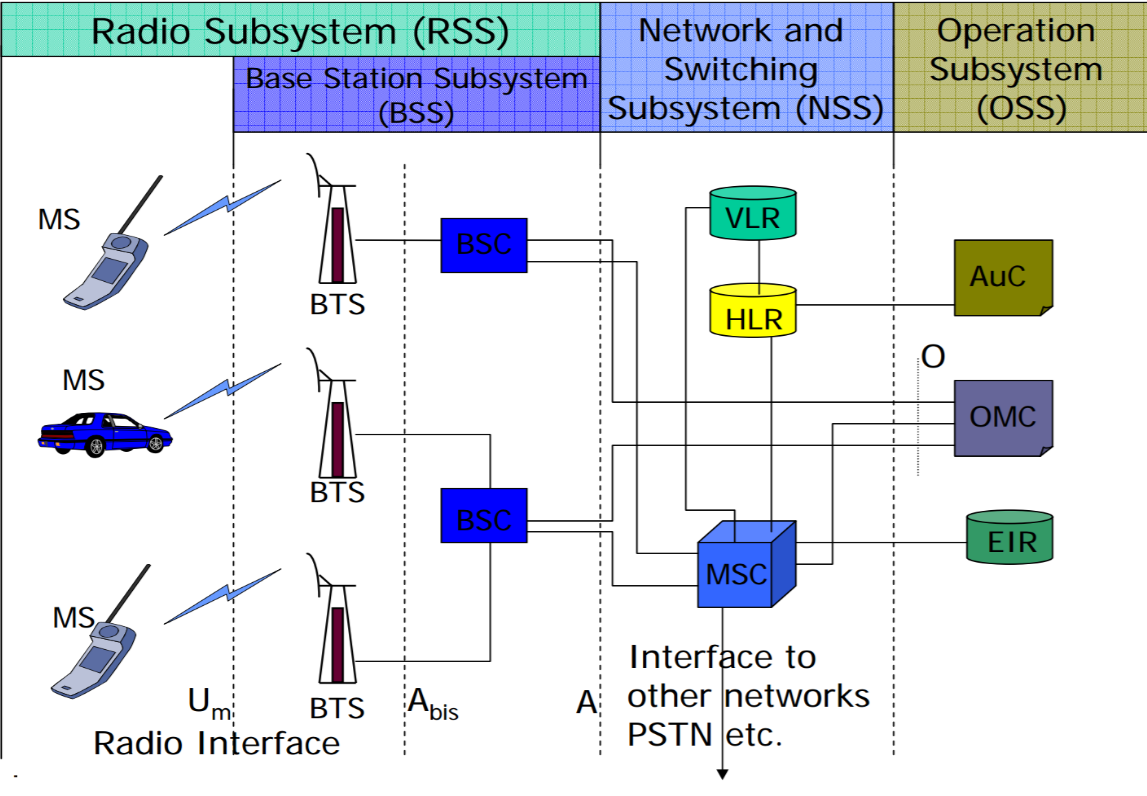
\includegraphics[scale=0.3]{archGSM.png}
  \caption{The structure of a GSM network}
  \label{fig:archGSM}
\end{figure}

\begin{itemize}
\item VLR : Visitor Location Register
\item HLR : Home Location Register
\item AUC : Authentication Center
\item BTS : Base Transceiver Station
\item OMC : Operation Maintenance Center
\item EIR : Equipment Identity Register
\end{itemize}
